\chapter{Platform}
\label{chap:platform}

$Crowdy$ is an extensible, general-purpose crowdsourcing platform to solve 
complex problems. The platform is developed over the fundamentals of stream 
processing paradigm for which a series of operations are applied to the continuous 
stream of data elements via operators.

$Crowdy$ is an operator-centric platform. Using this platform, a requester with no 
requirement of programming background can quickly translate a complex problem into 
a crowdsourcing application by simply selecting operators and connecting these operators 
together. As a result of $Crowdy$'s focus on operators, requesters can design applications 
by selecting right set of building blocks that are necessary to solve their problem, 
and customizing these blocks particular to the computation to-be-conducted.

$Crowdy$ embodies several features:
\begin{itemize}
	\item A standard toolkit of operators that can both human and software resources 
	(human or software) to accomplish various tasks
	\item Configuration support to control and coordinate resource utilization 
	\item Customizable collaborations over parameterization
	\item Application runtime interface
\end{itemize}

\section{Architecture}

$Crowdy$ platform is implemented as a REST~\cite{Richardson2008} architecture 
shown in Figure~\ref{fig:architecture}. Applications are developed, configured and 
validatedon the client-side. These applications are submitted to server-side via an 
application programming interface (API). Applications are executed, and results 
are saved on the server-side.

\begin{figure}[ht]
	\centering
	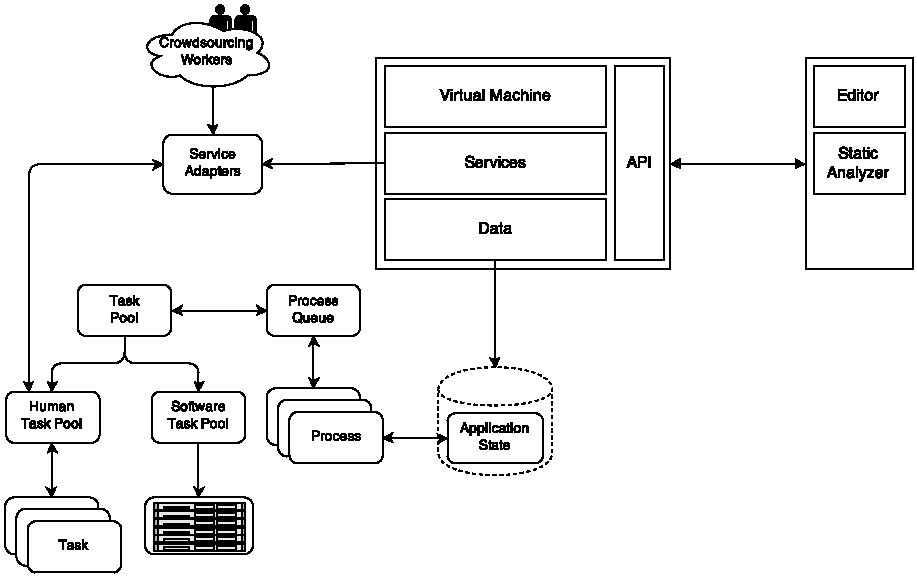
\includegraphics[height=200px]{figures/Architecture.pdf}
	\caption{Architecture of the platform.}
	\label{fig:architecture}
\end{figure}

The client-side provides an editor to easily create $Crowdy$ applications. Requesters 
can drag and drop various types of operators and connect them together to create a data 
flow, which conforms to a $Crowdy$ application. These applications are further analyzed 
and validated before submission. A valid application is submitted to the virtual machine 
on the server-side.

The server-side consists of three layers: virtual machine, services and data. In addition, 
an API is provided to submit new applications to the virtual machine and retrieve details 
of existing ones. Virtual machine sits on top of existing crowdsourcing services and 
provides service-independent environment for human computations. Once a new 
application is submitted, virtual machine first allocates required computation resources, 
then runs the application and finally saves the results. Services layer is formed by 
different crowdsourcing services such as Amazon's Mechanical Turk or microworkers. 
The data later is basically where application state is kept.

In the remainder of this chapter, the fundamental concepts of $Crowdy$ are explained 
in more detail and features are explored as we look into various aspects of application 
development using $Crowdy$ platform.

\section{Concepts}

$Crowdy$ applications are developed to solve complex and sophisticated problems 
that require both human intelligence and computing power. A typical application contains 
three main high-level components: data ingest, processing and data egress.

Let's consider a minimal "Hello World" application that has these three components 
in total, connected in a simple pipeline topology. Figure~\ref{fig:hello world} demonstrates 
the application in the form of a flow graph. On the ingest side, there is a 
\textit{source operator}, which acts like a data generator. Source operator produces 
data tuples that are processed down the flow by the 
\textit{processing operator}. Finally, the \textit{sink operator} simply converts the tuples 
in such a form (text file, email etc) that can be easily interpreted by requesters.

The application flow graph is specified as a series of operator instances and connections 
(data flows) that link them. A data flow basically transfers data tuples 
produced by an operator to another. One or more data segments can be assembled in a 
data tuple via output specification of an operator instance (see Section~\ref{sec:flow comp}). 
In addition, several options can be specified to configure an operator instance. These 
include parameters, operator-specific rules, which is studied in the rest of this chapter.

\begin{figure}[ht]
	\centering
	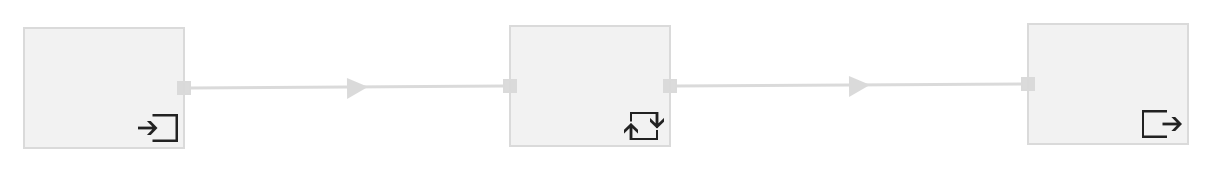
\includegraphics[width=0.85\textwidth]{figures/helloworld.png}
	\caption{A sample, minimal $Crowdy$ application.}
	\label{fig:hello world}
\end{figure}

In a more realistic application, one or more source operators can be employed to produce 
various data tuples that differ in both size and specification. Similarly, the application would 
have one or more processing operators along with other types of operators organized in a way 
that is significantly more complex than this example.

\subsection{Operator}
An operator is the basic building block of an application. Operator has a type that is 
specified at the time of creation. This type determines configuration respectively. Also a 
unique ID is assigned to an operator. In addition, operator has optional name and 
description fields that can be used for bookkeeping purposes.

\begin{figure}[ht]
	\centering
	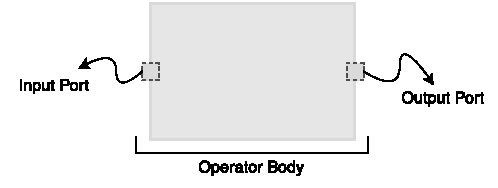
\includegraphics[height=100px]{figures/basicoperator.pdf}
	\caption{Base operator representation.}
	\label{fig:basic operator}
\end{figure}

Operator may have an input port or output port or both corresponding to it's type 
definition. Figure~\ref{fig:basic operator} demonstrates a base operator, which 
consists of a body and ports. Although it is not shown here, each operator presentation 
has a specific icon on their body associated with it's type.

An operator may output tuples to any number of operators, but it can only receive 
tuples from one operator unless it is a union operator (see Section~\ref{sec:utility operators}). 
However, union operator can only receive and aggregate tuples with same specification. 
Therefore, consistency of incoming flow specification for each operator type is ensured. 
This is a significant feature to guarantee operators functionality, because an operator 
most probably (excluding source operators) uses and operates on the information from 
incoming flow.

$Crowdy$ provides a set of built-in operators that can be used to build applications. 
In general, these operators perform common tasks associated with data generation, 
processing and outputting.

Operators are generally cross-domain to allow general-purpose 
computation possible. It is possible to group operators six main categories: 
\textit{source, sink, processing, relational, utility, adapter}.

\subsubsection{Source operators}
The set of source operators generates data tuples. These operators do not have 
an input port, but have an output port, which produces data tuples. Figure~\ref{fig:source operator} 
represents a source operator.

\begin{figure}[ht]
	\centering
	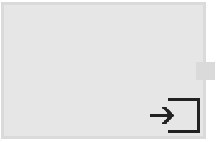
\includegraphics[height=60px]{figures/SourceOperator.pdf}
	\caption{Source operator representation.}
	\label{fig:source operator}
\end{figure}

Source operators together with processing operators are the ones that can be 
used to specify data flow coming out of an operator. Output specification is an 
action to identify the data tuple with a series of segments. Other operator types 
cannot make changes on output specification, but can manipulate the flow by dropping 
or copying data tuples.

\textbf{human.} 
The \textit{human source operator} is a stateless operator used to produce new data tuples 
via human workers. Existing crowdsourcing services such as MTurk is used 
to produce new tuples. A new data tuple is produced per successfully completed 
human intelligent task. These tasks are automatically created and posted with 
respect to the specified parameters of the operator.

Human source operator has the following parameters:
\begin{itemize}
	\item \texttt{number of copies}: The maximum number of data tuples can be 
	generated by the operator. It's value ranges from 1 to 1000.
	\item \texttt{max allotted time}: The maximum time in seconds given to a human 
	worker to solve and submit the task. It's value ranges from 10 to 300.
	\item \texttt{payment}: The payment in cents to be given to the human worker in 
	case of successful task completion. It's value ranges from 5 to 500.
	\item \texttt{instructions}: The detailed information for human workers on how to 
	complete the task.
	\item \texttt{question}: The set of sentences asking for specific information from 
	human workers.
	\item \texttt{input list}: The list of \texttt{input}s that will be shown to human worker 
	to fill in. An \texttt{input} can be a type of \textit{text, number, single choice} or 
	\textit{multiple choice}. Each of these types corresponds to an HTML element. 
	Table~\ref{tab:input list} lists types and their details.
	
	A text-input presents an input field where the human worker can 
	enter data. The maximum number of characters that can be entered to the field can be 
	set by the requester. Similarly number-input corresponds to a input field where only 
	numbers can be fed in, and the maximum and minimum value for the field are set by 
	the requester. The other two input types conform to input fields where the options given 
	by the requester are presented to the human worker as a list. Human worker is expected 
	to select only one and one or more options for single choice and multiple choice types 
	respectively.
	
	In fact, each \texttt{input} conforms to a segment in the data tuple.
\end{itemize}

\begin{table}[ht]
	\centering
	\caption{List of inputs and options}
	\label{tab:input list}
	\begin{tabular}{| l | l | l |}
		\hline
		type & parameters & HTML element \\ \hline
		text & max number of characters & input [type=text] \\ \hline
		number & min value, max value & input [text=number] \\ \hline
		single choice & options & input [type=radio] \\ \hline
		multiple choice & options & input [type=checkbox] \\ \hline
	\end{tabular}
\end{table} 


%This operator has a significant role in the platform. 
% platform-independence, abstracts away the details of the underlying platform
% use results of other operators
% customize collaboration by specifying audience

\textbf{manual.}
The \textit{manual source operator} is a stateless operator to produce new data 
tuples.

\newcommand{\ditto}{\texttt{\char`\'}}

Manual source operator has the following parameters:
\begin{itemize}
	\item \texttt{manual entry}: The manual text to be parsed and used to produce 
	new tuples.
	\item \texttt{delimiter}: Delimiter to determine segments in a tuple. This can have one 
	of the following values: none (\ditto\ditto), white space (\ditto\texttt{ }\ditto), 
	tab (\ditto\texttt{\char`\\t}\ditto), comma (\ditto\texttt{,}\ditto), 
	column (\ditto\texttt{:}\ditto).
\end{itemize}

Manual source operator uses manually entered text to create new tuples. Operator 
retrieves the manual text, parses it line by line and then applies the delimiter. 
Therefore, each line constitutes a data tuple, and delimiter is used to create segments 
in a tuple.

For example, if \texttt{delimiter} is chosen to be white space and the following is 
entered to \texttt{manual entry},

\begin{lstlisting}
Lorem ipsum
Consectetur adipiscing
Phasellus vehicula
\end{lstlisting}

\noindent the following data tuples will be generated:

\begin{lstlisting}
[
{"segment_1": "Lorem", "segment_2": "ipsum"},
{"segment_1": "Consectetur", "segment_2": "adipiscing"},
{"segment_1": "Phasellus", "segment_2": "vehicula"}
]
\end{lstlisting}

It is possible to have such a manual entry that ends up in different number of segments 
for different lines. To prevent this happening manual source operator uses the first line 
to generate output specification. If more segments are generated in the following lines, 
they are discarded. If there is not enough segments in another line, then the corresponding 
segments are emptied and then outputted.

\subsubsection{Sink operators}
The set of sink operators is where data tuples are serialized and converted into 
the formats that can be used by requesters with ease. These operators has one 
input port, but no output port. Figure \ref{fig:sink operator} demonstrates a sink operator.

\begin{figure}[ht]
	\centering
	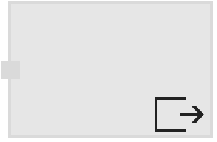
\includegraphics[height=60px]{figures/SinkOperator.pdf}
	\caption{Sink operator representation.}
	\label{fig:sink operator}
\end{figure}

\textbf{email.}
The \textit{email sink operator} is a stateless operator to convert data tuples into a 
text format and email them to requesters. \texttt{email} parameter specifies the 
requester's email address. 

\textbf{file.}
The \textit{file sink operator} is a stateless operator to serialize the data tuples into 
a file. Operator has one parameter \texttt{filename} that is used to specify the name 
of file in which tuples will be written.

\subsubsection{Processing operators}
The set of processing operators provides data tuple processing via human workers. 
These operators have both input and output ports. Figure \ref{fig:processing operator} 
shows a processing operator.

\begin{figure}[ht]
	\centering
	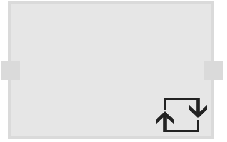
\includegraphics[height=60px]{figures/ProcessingOperator.pdf}
	\caption{Processing operator representation.}
	\label{fig:processing operator}
\end{figure}

As mentioned before, processing operators can manipulate the data flow specification 
in addition to source operators. These operators can change the existing flow specification 
by adding, deleting or editing data segments.

\textbf{human.}
The \texttt{human processing operator} is almost same as human source operator. 
The difference is human processing operator has an input port. That means there is a 
flow of data tuples coming to operator. These incoming tuples are made available 
to requesters via their specification.

The parameters of human processing operator is no different than the parameters of 
human source operator. Additionally processing operator has available segment list, which 
provides placeholders for the segments of an incoming data tuple. Requesters can place 
these placeholders in \texttt{instructions}, \texttt{question} and \texttt{input list} 
(applicable to single choice and multiple choice inputs).

At runtime when a new tuple arrives, each placeholder in parameters is replaced with 
the corresponding value of incoming tuple's segment. This enables dynamically created human 
tasks. Therefore, requesters can create an information flow from one operator to another.

\subsubsection{Relational operators}
The set of relational operators enables fundamental manipulation operations on 
the flow of data tuples. Each relational operator implements a specific functionality 
providing continuous and non-blocking processing on tuples. Therefore, these operators 
have both input and output port.

\textbf{selection.}
The \textit{selection operator} is a stateless operator used to filter tuples. A typical 
selection operator is shown in Figure~\ref{fig:selection operator}.

\begin{figure}[ht]
	\centering
	
\includegraphics[height=60px]{figures/SelectionOperator.pdf}
	\caption{Selection operator representation.}
	\label{fig:selection operator}
\end{figure}

On a per-tuple basis a boolean predicate is evaluated and a decision is made as 
to whether to filter the corresponding tuple or not. Boolean predicates are specified 
by requesters as part of operator parameterization. These predicates, which are 
identified in \texttt{rules}, are the only members of parameters.

A selection operator has zero or more rules to filter data tuples. When there is 
no rule specified, then no filtering will be done, and all data tuple will be passed 
down to data flow. Otherwise, each rule is evaluated on an incoming data tuple. 
Whenever a rule is evaluated to be true, then corresponding action is carried out 
that is either filter in or out the tuple. If no rule is evaluated to be true on a data tuple, 
then tuple is still passed to the next operator. Rules share the following predefined 
format:

\textit{Filter} \textit{(in/out)} \textit{when} \texttt{boolean-predicate}

Similarly \texttt{boolean-predicate} has the following format

\texttt{segment-name} \textit{(equals/not equals/contains)} \texttt{query}

where \texttt{segment-name} is one of the segments of incoming tuple, 
and \texttt{query} is a free-text to be filled by requester.

\textbf{sort.}
The \textit{sort operator} is a stateful and windowed operator used to first group 
tuples and then sort them based on the specified data segment and order. Figure
~\ref{fig:sort operator} illustrates the operator.

\begin{figure}[ht]
	\centering
	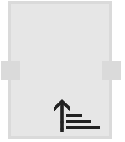
\includegraphics[height=60px]{figures/SortOperator.pdf}
	\caption{Sort operator representation.}
	\label{fig:sort operator}
\end{figure}

Sorting is performed and results are produced (outputted one by one) every time 
window trigger policy fires. The policy is basically triggered when the number of 
data tuples reaches \texttt{window size}, which is specified as a parameter. 
\texttt{window size} can have a value between 1 and 100.

Similar to selection operator, sort operator implements a set of rules that simply 
identifies the segment and the order to be used for sorting. If no rule is specified, 
then tuples are sorted in the ascending order with respect to the first segment in 
the incoming data tuples. If there are more than one rule is given, then these rules 
are applied in the order they are specified by requester.

Sorting rules share the following predefined format:

\textit{Sort using} \texttt{segment-name} \textit{in} \textit{(ascending/descending)} \textit{order}

where \texttt{segment-name} is one of the segments of incoming tuple.

\subsubsection{Utility operators}
\label{sec:utility operators}
The set of utility operators provides flow management functions. These operators 
handle operations such as separating a flow into multiple flows or joining multiple 
flows into a single one.

\textbf{enrich.}
The \textit{enrich operator} is a stateless operator used to enrich data flow by 
replaying incoming data tuples. Figure~\ref{fig:enrich operator} shows an example 
view of the operator.

\begin{figure}[ht]
	\centering
	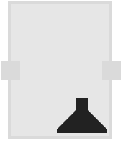
\includegraphics[height=60px]{figures/EnrichOperator.pdf}
	\caption{Enrich operator representation.}
	\label{fig:enrich operator}
\end{figure}

Enrich operator has one parameter called \texttt{number of copies}. This parameter 
determines how many copies will be produced for each incoming tuple. It's value 
ranges from 1 to 10.

\textbf{split.}
The \textit{split operator} is a stateless operator used to divide an inbound flow 
into multiple flows. This operator has one incoming flow and and can have one or 
more outgoing flow. Figure~\ref{fig:split operator} provides the presentation of a 
split operator.

\begin{figure}[ht]
	\centering
	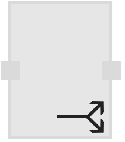
\includegraphics[height=60px]{figures/SplitOperator.pdf}
	\caption{Split operator representation.}
	\label{fig:split operator}
\end{figure}

The boolean predicates specified in rules are evaluated whenever a new tuple 
arrives. Then, a decision is made to where to send the tuple. Similar to relational 
operators, rules are specified by requesters as part of operator 
parameterization.

A split operator has zero or more rules. When there is no rule specified, then 
tuples are passed to every operator connected down the flow. Otherwise, each 
and every rule is evaluated on an incoming data tuple. Whenever rule's predicate 
is evaluated to be true, then tuple is passed to the corresponding operator. If no 
predicate turns out to be true for a tuple, then it is dropped.

Rules share the following predefined format:

\textit{Send to} \texttt{next-operator} \textit{when} \texttt{boolean-predicate}

in which \texttt{next-operator} is the connected operators down the flow, and 
\texttt{boolean-predicate} has the same definition given for selection operator.

\textbf{union.}
The \textit{union operator} is a stateless operator used to join two or more data flows 
into one. Different than other operators, this operator can receive more than one flow. 
These flows are combined by the operator and outputted as if they are a single flow. 
Figure~\ref{fig:union operator} demonstrates the operator.

\begin{figure}[ht]
	\centering
	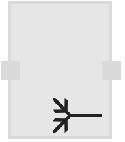
\includegraphics[height=60px]{figures/UnionOperator.pdf}
	\caption{Union operator representation.}
	\label{fig:union operator}
\end{figure}

Union operator requires incoming flows to have the same specification. Otherwise, 
union operation will basically fail.

\section{Flow compositon}
\label{sec:flow comp}
TODO